% \iffalse
\let\negmedspace\undefined
\let\negthickspace\undefined
\documentclass[journal,12pt,twocolumn]{IEEEtran}
\usepackage{cite}
\usepackage{amsmath,amssymb,amsfonts,amsthm}
\usepackage{algorithmic}
\usepackage{graphicx}
\usepackage{textcomp}
\usepackage{xcolor}
\usepackage{txfonts}
\usepackage{listings}
\usepackage{enumitem}
\usepackage{mathtools}
\usepackage{gensymb}
\usepackage{comment}
\usepackage[breaklinks=true]{hyperref}
\usepackage{tkz-euclide} 
\usepackage{listings}
\usepackage{gvv}                                        
\def\inputGnumericTable{}                                 
\usepackage[latin1]{inputenc}                                
\usepackage{color}                                            
\usepackage{array}                                            
\usepackage{longtable}                                       
\usepackage{calc}                                             
\usepackage{multirow}                                         
\usepackage{hhline}                                           
\usepackage{ifthen}                                           
\usepackage{lscape}
\newtheorem{theorem}{Theorem}[section]
\newtheorem{problem}{Problem}
\newtheorem{proposition}{Proposition}[section]
\newtheorem{lemma}{Lemma}[section]
\newtheorem{corollary}[theorem]{Corollary}
\newtheorem{example}{Example}[section]
\newtheorem{definition}[problem]{Definition}
\newcommand{\BEQA}{\begin{eqnarray}}
\newcommand{\EEQA}{\end{eqnarray}}
\newcommand{\define}{\stackrel{\triangle}{=}}
\theoremstyle{remark}

\newtheorem{rem}{Remark}
\begin{document}
\parindent 0px
\bibliographystyle{IEEEtran}
\title{Assignment 11.9.5\_6Q}
\author{EE23BTECH11028 - Kamale Goutham$^{}$% <-this % stops a space
}
\maketitle
\newpage
\bigskip
\section*{Question}
Find the sum of all two digit numbers which when divided by $4$,yields $1$ as reminder?\\
\solution 
Input parameters are:\\
\begin{table}[ht]
    \centering
    \def\arraystretch{1.5}
    \footnotesize
\begin{tabular}{|p{2cm}|p{2.5cm}|p{2.3cm}|}
    \hline
    PARAMETER & VALUE & DESCRIPTION  \\ \hline
    $$x\brak0$$ & $$13$$ & First term \\ \hline
    $$d$$ & $$4$$ & common difference \\ \hline
    $$x(n)$$ & $$[13+4n]u\brak n$$ & General term of the series  \\ \hline
  \end{tabular}

    \caption{INPUT PARAMETER TABLE}
    \label{tab:11.9.5.6}
\end{table}
  \begin{align}
    \text{x(n)}=&x(0)+n{\text{d}}\\
    n=&\frac{97-13}{4}=21\\
X(z)=&\sum\limits^{\infty}_{k=-\infty}{x(k)\times u(k)\times(z^{-k}})\\
\implies    n u\brak{n} & \system{Z} \frac{z^{-1}}{\brak{1-z^{-1}}^2} ,   \abs{z} >1 \\
X(z)=&\frac{13-9z^{-1}}{(1-z^{-1})^2},|z|>1\\
y(n)=&x(n)*u(n)\\ Y(z)=&X(z)U(z)\\\implies Y(z)=&\brak{\frac{13-9z^{-1}}{(1-z^{-1})^{3}}},|z|>1
\end{align}
Using contour integration to find the inverse z-transform,
\begin{align}
    y(n)=&\frac{1}{2\pi j}\oint_{C}Y(z) z^{n-1} dz  \\y(21)=&\frac{1}{2\pi j}\oint_{C}\brak{\frac{(13-9z^{-1})z^{20}}{(1-z^{-1})^{3}}}
\end{align}
We can observe that the pole is repeated $3$ times and thus $m=3$,
\begin{align}
    R&=\frac{1}{\brak {m-1}!}\lim\limits_{z\to a}\frac{d^{m-1}}{dz^{m-1}}\brak {{(z-a)}^{m}f\brak z}  \\&=\frac{1}{\brak {2}!}\lim\limits_{z\to 1}\frac{d^{2}}{dz^{2}}\brak{13z^{23}-9z^{22}}\\R&=1210\\
        \therefore &y\brak{21}=1210
\end{align}
Therefore, the sum of all two-digit numbers that, when divided by 4, yield a remainder of 1 is 1210.\\
\begin{figure}[h]
  \centering
  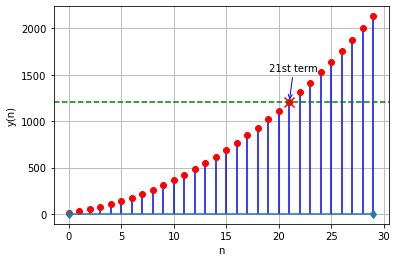
\includegraphics[width=\columnwidth]{Graph/plot1.png}
  \caption{y(n) = $13 + 15n+2n^2$}
  \label{fig:graph}
\end{figure}
\end{document}
